\documentclass[11pt]{article}
\usepackage[margin=1in]{geometry}
\usepackage[T1]{fontenc}
\usepackage[utf8]{inputenc}
\usepackage{lmodern,amsmath,amssymb,amsthm,booktabs,array,tikz}
\usepackage[title]{appendix}
\usepackage{float,needspace}
\usepackage[hyphens]{url}
\usepackage[colorlinks=true,linkcolor=blue,citecolor=blue,urlcolor=blue]{hyperref}
\newtheorem{theorem}{Theorem}[section]
\newtheorem{proposition}[theorem]{Proposition}
\newtheorem{lemma}[theorem]{Lemma}
\theoremstyle{definition}
\newtheorem{definition}[theorem]{Definition}
\newcommand{\C}{\mathbb C}
\newcommand{\NC}{\operatorname{NC}}
\newcommand{\rank}{\operatorname{rank}}
\newcommand{\Fix}{\operatorname{Fix}}
\setlength{\emergencystretch}{2em}
\raggedbottom
\widowpenalty=10000
\clubpenalty=10000
\title{Symmetric chains in noncrossing partition lattices}
\author{P. Graham\\ \small\url{https://orcid.org/0009-0007-8493-1505}}
\date{October 25, 2026}
\hypersetup{pdfauthor={P. Graham},pdftitle={Symmetric chains in noncrossing partition lattices}}
\begin{document}
\maketitle
\begin{abstract}
Every noncrossing partition lattice of a finite well-generated complex
reflection group admits a symmetric chain decomposition. We give a
computer-assisted proof for the exceptional types $H_4$, $G_{33}$,
$G_{34}$, $E_6$, $E_7$, and $E_8$, completing the saturated-chain
assertion asked by Henri M\"uhle. Simion and Ullman, Reiner, Bessis
and Corran, and M\"uhle established the other irreducible cases.
Explicit chain certificates are checked against exact reflection-group
models; exhaustive rank descent certifies that their graphs are the full
absolute-order intervals. Reflection-preserving automorphisms and a
constructive product decomposition give every Coxeter element and every
reducible group. Lean verifies the general interval-closure, product,
and transfer lemmas. The finite group calculations and the published
classification and decomposition results remain external inputs.
\end{abstract}


\section{Introduction}
A noncrossing partition of a circularly ordered set groups its points
into blocks whose convex hulls do not cross. Ordering these partitions
by refinement gives the classical noncrossing partition lattice. Its
generalization to reflection groups replaces refinement by absolute
order: an element lies below another when a shortest reflection
factorization can be extended to one for the latter. We prove the
following statement; the terminology is made precise below.
The partition it describes is a symmetric chain decomposition.

\begin{theorem}\label{thm:main}
Let $W$ be a finite well-generated complex reflection group of essential
rank $n$. For each irreducible factor choose any Coxeter element, and
let $c$ be their product. The noncrossing partition lattice
$\NC(W,c)$ has a partition into nonempty saturated chains whose
bottom and top ranks sum to $n$. The trivial group, of rank zero, is
included.
\end{theorem}

The new contribution is the chain decomposition for the six exceptional
types named in the abstract. The main difficulty is the compatibility
of chains across every rank: rank symmetry, unimodality, and the strong
Sperner property do not supply such chains. M\"uhle's work already
established those properties for all well-generated groups
\cite[Theorem~1.4]{Muhle}. Here explicit partitions supply the missing
chain decompositions. Their discovery uses Griggs's matching
construction, iterated from the middle ranks as in Tomon's work
\cite{Griggs,Tomon}. Their verification also establishes the complete
interval and its covers, rather than relying on a graph with the
expected number of vertices.

\begin{samepage}
\subsection*{The question and earlier work}
Henri M\"uhle asks \cite[Question~1.1]{Muhle}:
\begin{quote}
Does the lattice of $W$-noncrossing partitions always admit a symmetric
decomposition into saturated chains or Boolean lattices for every
well-generated complex reflection group $W$?
\end{quote}
\end{samepage}
Theorem~\ref{thm:main} answers its chain part. The Boolean part is
not settled here.

Rodica Simion and Daniel Ullman constructed symmetric decompositions
for classical noncrossing partitions \cite{SU}. Victor Reiner proved
the type-$B$ chain assertion \cite[Theorem~13]{Reiner}; Patricia Hersh's
local symmetric-group actions give the stronger Boolean decomposition
in type $B$ \cite[Theorems~5 and~7]{Hersh}. David Bessis and Ruth Corran
identify the $G(d,1,m)$ intervals with type $B$ for $d\geq2$ \cite{BC}.
M\"uhle proves the Boolean assertion for $G(d,d,m)$ and the chain
assertion for the small exceptional types, leaving the six treated here
\cite[Theorem~1.3 and Proposition~4.2]{Muhle}. He also records an earlier
unpublished type-$D$ chain construction by Eleni Tzanaki
\cite[introduction, after Theorem~1.3]{Muhle}.

The reduction uses the classification of Geoffrey Shephard and John
Todd \cite{ST}. The exact models use the Coxeter representations
described by Drew Armstrong \cite{Armstrong}, the invariant degrees
tabulated by David Bessis \cite{Bessis}, and the Coxeter--Todd root
coordinates and named generators described by Manabu Oura and Jiro
Sekiguchi \cite{OS}, building on John Conway and Neil Sloane \cite{CS}.
The passage between all choices of Coxeter element uses the theorem of
Victor Reiner, Vivien Ripoll, and Christian Stump \cite{RRS}.

Recent related work includes Michael Dougherty and Gina Root's
symmetric chain results under conditions on planar hull configurations
\cite[Theorem~A]{DR}, and Alice Gao, Xin-Bei Liu, Arthur Yang, and James Zhao's
interlacing symmetric decompositions of order-complex $h$-polynomials
\cite[Theorem~1.5]{GLYZ}. The former concerns a geometric class of partition
lattices; the latter decomposes polynomials rather than the elements
of an absolute-order interval. These results address different
extensions of classical noncrossing-partition structure.
For general graded posets, Nate Harman, Rylan Rosas, Charles
Troutman~III, and Chris Wu introduce strong $\mathfrak{sl}_2$-actions
and conjecture their equivalence with symmetric chain decompositions
\cite[Definition~1.1 and Conjecture~1.2]{HRTW}. The certificates here give the chains directly and do
not require that conjecture.

The proof combines exact finite computations with the general lemmas
checked in Lean; Section~\ref{sec:checking} describes their relation.

The proofs, the Lean formalization, the certificate checkers and the text were produced by AI models (from OpenAI and Anthropic), working under the author's direction. This computer-assisted work has not yet been reviewed by experts.

\section{Definitions and proof overview}\label{sec:overview}
We recall the conventions and then describe the argument.

A \emph{complex reflection} on a finite-dimensional complex vector
space $V$ is a nonidentity finite-order linear transformation fixing
a hyperplane pointwise. A finite complex reflection group is a finite subgroup of $\operatorname{GL}(V)$
generated by reflections. Its \emph{essential rank} is
$\dim V-\dim\Fix(W)$. It is \emph{well-generated} if it can be generated
by that many reflections. A fixed summand can be removed without
changing any reflection length below.

Let $T$ be the set of all reflections in $W$. It is closed under
inversion and conjugation. The \emph{reflection length} $\ell_T(w)$ is
the smallest number of factors from $T$ in a product equal to $w$.
The \emph{absolute order} and its interval below $c$ are
\begin{align*}
 u\leq_T v&\quad\Longleftrightarrow\quad
       \ell_T(u)+\ell_T(u^{-1}v)=\ell_T(v),\\
 \NC(W,c)&=[1,c]_T.
\end{align*}
The rank of an element in this interval is $\ell_T(w)$.

For the essential rank-$n$ representation, the algebra of invariant
polynomials $\C[V]^W$ is a polynomial algebra on $n$ homogeneous
generators. Their degrees $d_1\leq\cdots\leq d_n$ are independent
of the choice of homogeneous generators and are called the
\emph{invariant degrees} of $W$. For irreducible $W$, let $h=d_n$
be the largest invariant degree. A vector
is \emph{regular} if it lies outside every reflecting hyperplane. A
\emph{Coxeter element} here means a regular element of order $h$: it
has an eigenvector that is regular, with eigenvalue of order $h$.
This includes every regular element of order $h$, not just one
conjugacy class. For a reducible group the choice is componentwise,
as in Theorem~\ref{thm:main}.

For example, $\NC(S_3,(123))$ has rank sizes $1,3,1$. A maximal chain
$1<(12)<(123)$, together with the two singleton chains $(13)$ and
$(23)$, is a symmetric chain decomposition. The maximal chain has
endpoint ranks $0,2$, and each singleton has rank $1$.

\begin{definition}
In a finite graded poset of rank $n$, a \emph{saturated chain} has a
cover relation between each consecutive pair. It is \emph{symmetric}
if its endpoint ranks sum to $n$. A \emph{symmetric chain
decomposition} is a partition of the elements into nonempty symmetric
saturated chains.
\end{definition}

The proof has three parts. First, published decompositions leave only
six irreducible types. For one Coxeter element in each type, the supplied
certificates list the chains by exact matrix labels. Second, a complete
reflection census and exhaustive downward reflection steps identify the
certified graph with $[1,c]_T$. The key observation is that, on a
reflection walk of length $n$ from $c$ to $1$ with
$\rank(I-c)=n$, the quantity $\rank(I-w)$ must drop at every step.
This turns interval completeness into a finite closure check.
Finally, reflection-preserving automorphisms transport the chains to
every Coxeter element, and a grid construction combines factor chains
for reducible groups.

The argument does not assume that reflection length equals fixed-space
codimension on the entire complex reflection group. It proves that
equality only for the certified interval.

\section{Absolute-order intervals}\label{sec:finite}
The finite criterion below applies in any faithful finite-dimensional
representation.

Put $q(w)=\rank(I-w)$. The identity
\[
                    I-uv=(I-u)+u(I-v)
\]
implies $q(uv)\leq q(u)+q(v)$. In particular
\begin{equation}\label{eq:qbound}
 q(w)\leq\ell_T(w),\qquad q(w)\leq q(wt)+1\quad(t\in T).
\end{equation}
The second inequality follows by applying subadditivity to
$w=(wt)t^{-1}$. A \emph{reflection walk} has steps
$w\longmapsto wt$ with $t\in T$.

\begin{lemma}\label{lem:walk}
Suppose $q(c)=n$ and $c$ has a reflection word of length $n$.
Then $\ell_T(c)=n$. An element $x$ belongs to $[1,c]_T$ if and only
if it lies on a reflection walk from $c$ to $1$ of length $n$.
Every step of every such walk lowers $q$ by one. At any vertex $x$
on the walk, $q(x)=\ell_T(x)$.
\end{lemma}
\begin{proof}
The word and \eqref{eq:qbound} give
$n=q(c)\leq\ell_T(c)\leq n$.
If $x\leq_T c$, reduced words for $x^{-1}c$ and $x$, removed in
reverse order, give a right-reflection walk $c\to x\to1$ of total
length $n$. Conversely, if such a walk takes $k$ steps to reach $x$
and $n-k$ more to reach $1$, then
\[
 \ell_T(x^{-1}c)\leq k,\qquad \ell_T(x)\leq n-k.
\]
The triangle inequality for reflection length forces their sum to be
$n$, so $x\leq_T c$.

The $n$ steps lower $q$ from $n$ to zero. By \eqref{eq:qbound} each
step lowers it by at most one. The sum of these decreases is $n$,
so each is one. Thus $q(x)=n-k$. Since
$q(x)\leq\ell_T(x)\leq n-k$, equality holds.
\end{proof}

\begin{proposition}[Finite interval criterion]\label{prop:criterion}
Suppose $T$ is the entire reflection set, $q(c)=n$, and a reflection
word of length $n$ for $c$ is supplied. Let $S$ be a finite set of
distinct elements of $W$ containing $c$ and $1$. Suppose that:
\begin{enumerate}
\item each $x\in S$ lies on a reflection walk $c\to x\to1$ of total
      length $n$;
\item for each $x\in S$ and $t\in T$, if $q(xt)=q(x)-1$, then
      $xt\in S$.
\end{enumerate}
Then $S=[1,c]_T$, and $q$ is its absolute-order rank. Its downward
covers are exactly the pairs $x\longmapsto xt$ with $x,xt\in S$ and
$q(xt)=q(x)-1$.
\end{proposition}
\begin{proof}
The first condition and Lemma~\ref{lem:walk} give
$S\subseteq[1,c]_T$ and $q=\ell_T$ on $S$. If $y\in[1,c]_T$,
choose a length-$n$ walk through $y$. Every step lowers $q$ by one.
Starting at $c\in S$, the second condition keeps that walk in $S$;
hence $y\in S$.

For a pair in the asserted downward edge set, write $y=xt$.
The equality $\ell_T(y)=\ell_T(x)-1$ and the fact that
$y^{-1}x=t^{-1}$ is a reflection give $y<_T x$. Their ranks differ
by one, so this is a cover. Conversely, if $y<_T x$, a reduced word
for $y^{-1}x$ extends a reduced word for $y$ to one for $x$.
Its successive prefixes give all intervening absolute ranks. They
also lie below $c$, by extending further to a reduced word for $c$.
If $y<_T x$ is a cover, there can therefore be only one added
reflection. This is precisely a downward reflection step of rank one.
\end{proof}

The criterion certifies vertices and covers together. Checking only
cardinality, or checking chains on two copies of the same incomplete
graph, would not establish either conclusion.

\section{The exceptional cases}\label{sec:models}
The six certificates use the exact reflection-group models specified
in Appendix~\ref{app:models}. We explain why their checks establish
Proposition~\ref{prop:criterion}.
The complete chain partitions and reflection words are in the
\href{https://doi.org/10.5281/zenodo.23605555}{archived verification package}.

The chains use Griggs's matching construction \cite{Griggs} in the
iterative form described by Tomon \cite[\S\S3--4]{Tomon}. It starts
with singleton chains in the middle rank when the total rank is
even, or a perfect matching between the two middle ranks when it
is odd. At each
stage, a bipartite perfect matching either extends a chain at both
ends by one cover or leaves it finished. Two copies of each active
chain, joined by an identity edge, allow these choices in a single
matching problem.

\subsection{Reflections and Coxeter elements}
The root formulas provide a candidate reflection set. Its completeness
is checked independently of the formula: the checker computes all
conjugacy classes of the generated group, tests $\rank(I-g)$ on every
class representative, and requires every member of every rank-one class
to occur in the candidate set. Rank is constant on a conjugacy class.
The class sizes must sum to the group order. Thus this step establishes
the entire reflection set, subject to the exact group algorithms
described in Section~\ref{sec:checking}. In these six groups the
reflections are involutions; no such restriction is imposed on the
published family inputs.

The selected element $c$ is supplied as a word in $n$ reflections.
The checker verifies $q(c)=n$, its order $h$, and an exact eigenvector
for $e^{2\pi i/h}$ that is fixed by none of the reflections. This last
test puts the eigenvector outside every reflecting hyperplane, so
establishes regularity. The invariant degrees, and hence the relevant
values of $h$, are taken from \cite[Table~2]{Bessis}; they are not
inferred from an observed group order. Table~\ref{tab:finite} records
the parameters and sizes of the certificates.



\subsection{Interval and chain verification}
For each group the interval generator starts from $c$ and tests every
right multiplication by a reflection, retaining exactly the rank
descents. It does not read the chain partition. A separately written
semantic checker reconstructs the supplied vertices and computes ranks
by its own exact row elimination. For every vertex $x$ and every
reflection $t$, it checks the downward-closure condition and requires
that the recorded edges are exactly all resulting pairs.

The checker also verifies paths from $c$ to every vertex and from every
vertex to $1$. Every edge lowers $q$ by one, so these paths have
total length $n$. Strictly decreasing ranks make the path verification
noncircular. All hypotheses of Proposition~\ref{prop:criterion} are
therefore checked. The resulting graph is the full absolute-order
interval with its actual covers.

The chain files use the same exact basis-image labels. Two independent
chain checkers, written in Python and JavaScript, require each chain to
be nonempty, every vertex to occur exactly once, consecutive vertices
to be recorded covers of successive ranks, and endpoint ranks to sum
to $n$. These conditions are the definition of a symmetric chain
decomposition.

\begin{proposition}\label{prop:six}
For each of $H_4,G_{33},G_{34},E_6,E_7,E_8$, the supplied certificates
give a symmetric chain decomposition of $\NC(W,c)$ for the chosen
Coxeter element $c$.
\end{proposition}
\begin{proof}
The exact checks just described establish the hypotheses of
Proposition~\ref{prop:criterion} and every condition in the definition
of a symmetric chain decomposition. All six certificates pass these
checks.
\end{proof}

\section{From six types to all groups}\label{sec:reduction}
We assemble the finite inputs with the published cases, and prove the
two elementary transfer steps needed for the full statement.

\subsection{Irreducible groups}
Write $G(r,p,m)$ for the monomial group whose nonzero entries are
$r$th roots of unity and whose product of nonzero entries is an
$(r/p)$th root of unity, where $p\mid r$. The well-generated filter
of the Shephard--Todd classification \cite{ST}, as stated in
\cite[\S2.2]{Muhle}, leaves the families and exceptional types below.
The classification and filter are published inputs, not consequences
of the certificate computations.

The family $G(1,1,m)$ is $S_m$, with essential rank $m-1$ in its
permutation representation. Its noncrossing interval is the classical
lattice, and the result is Simion--Ullman's theorem \cite[Theorem~2]{SU},
restated in \cite[Theorem~3.6 and Corollary~3.7]{Muhle}.
For $d\geq2$, Bessis--Corran's remark at the end of \S7 and their
paragraph after Corollary~8.2 identify $\NC(G(d,1,m))$ with the
type-$B$ interval \cite{BC}. Reiner's Theorem~13 supplies its chain
decomposition \cite{Reiner}. For $d,m\geq2$, the
$G(d,d,m)$ case is \cite[Theorem~1.3]{Muhle}.
The reducible parameter $G(2,2,2)$ is also covered by the product
argument below.
A symmetric Boolean piece is refined into symmetric chains by the
product construction of Lemma~\ref{lem:product}; this explains the
Boolean-to-chain implication used in the cited family cases
\cite[Proposition~2.1]{Muhle}.

There are $26$ exceptional well-generated types, with indices
\[
 4,5,6,8,9,10,14,16,17,18,20,21,23,24,25,26,27,28,29,30,
 32,33,34,35,36,37.
\]
Of these, Proposition~4.2 of \cite{Muhle} covers the twenty types
\[
 4,5,6,8,9,10,14,16,17,18,20,21,23,24,25,26,27,28,29,32.
\]
The remaining six are exactly those in Proposition~\ref{prop:six}.
In particular $G_{32}$ has rank four and belongs to the cited cases.
This proves the chain assertion for one Coxeter element in every
irreducible type. Rank-one groups are cyclic; all their nonidentity
elements are reflections, and their interval is the single chain
$1<c$. The rank-zero interval is a singleton.

\subsection{Every choice of Coxeter element}
Theorem~\ref{thm:main} allows all Coxeter elements in the regular-element
sense. By Reiner--Ripoll--Stump \cite[Proposition~1.4 and Corollary~1.5]{RRS},
for any two Coxeter elements $c,c'$ of an irreducible well-generated
group there is a group automorphism $\phi$ with
$\phi(T)=T$ and $\phi(c)=c'$. Applying $\phi$ to a shortest
reflection word, and then doing the same with $\phi^{-1}$, proves
\[
                       \ell_T(\phi(w))=\ell_T(w).
\]
The defining equality for absolute order now gives
\[
 u\leq_T v\ \Longleftrightarrow\ \phi(u)\leq_T\phi(v).
\]
Thus $\phi$ restricts to a rank-preserving order isomorphism
$[1,c]_T\to[1,c']_T$. An order isomorphism preserves covers,
partitions, and endpoint ranks; it carries a symmetric chain
decomposition to one for $c'$. This uses a reflection-preserving
automorphism, not an assertion that all Coxeter elements are conjugate
inside $W$.

\subsection{Products of groups and chains}
For the essential product representation $W=W_1\times W_2$,
fixed-space codimensions add. A reflection of $W$ is consequently
exactly $(t,1)$ or $(1,u)$ with $t$ or $u$ a reflection in its
factor. Projecting any reflection word and concatenating shortest
factor words give the two inequalities proving
\begin{equation}\label{eq:productlength}
 \ell_T((x,y))=\ell_{T_1}(x)+\ell_{T_2}(y).
\end{equation}
For each factor, the triangle inequality says
\[
 \ell_{T_i}(x_i)+\ell_{T_i}(x_i^{-1}c_i)\geq\ell_{T_i}(c_i).
\]
By \eqref{eq:productlength}, the absolute-order equality for the
product holds exactly when both factor inequalities are equalities.
The same calculation for two arbitrary product elements shows that
their absolute order is coordinatewise. Hence
\begin{equation}\label{eq:intervalproduct}
 [1,(c_1,c_2)]_T=[1,c_1]_{T_1}\times[1,c_2]_{T_2}
\end{equation}
as ranked posets, with ranks added.

The standard product construction is due to de Bruijn, van Ebbenhorst
Tengbergen, and Kruyswijk \cite{BTK}; see also Srinivasan's account
\cite[\S1]{Srinivasan}.

\begin{lemma}\label{lem:product}
The product of two finite graded posets with symmetric chain
decompositions has a symmetric chain decomposition.
\end{lemma}
\begin{proof}
Partition the product into products of factor chains. Take chains
with bottom ranks $p,q$ and lengths in steps $a,b$. Their product
is a grid $[0,a]\times[0,b]$ whose element $(i,j)$ has rank
$p+q+i+j$. For each integer $0\leq k\leq\min(a,b)$ take
\begin{equation}\label{eq:grid}
 (k,0),(k,1),\ldots,(k,b-k),
 (k+1,b-k),\ldots,(a,b-k).
\end{equation}
Empty final portions are omitted. A vertex $(i,j)$ lies on exactly
the chain with label $\min(i,b-j)$: when $i\leq b-j$ it is on
the vertical portion, and when $i>b-j$ it is on the horizontal
portion. These chains therefore partition the grid.

Each step increments exactly one coordinate and is a cover in its
factor, so is a cover in the product poset. The endpoint ranks are
$p+q+k$ and $p+q+a+b-k$. Their sum is
$(2p+a)+(2q+b)$, the sum of the factor ranks by symmetry of the
factor chains. Thus every chain is symmetric in the product.
\end{proof}

\begin{figure}[ht]
\centering
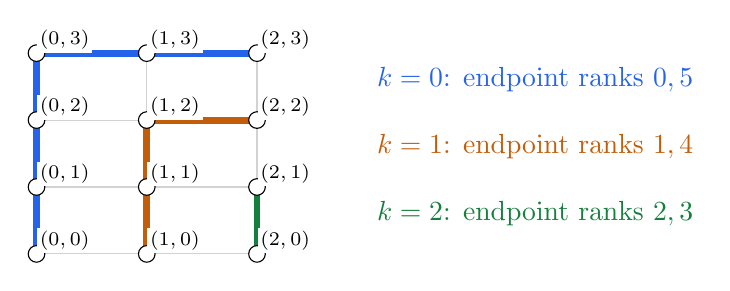
\begin{tikzpicture}[x=1.4cm,y=0.85cm]
 \definecolor{chainblue}{HTML}{2563EB}
 \definecolor{chainorange}{HTML}{C45D0A}
 \definecolor{chaingreen}{HTML}{15803D}
 \foreach \i in {0,1,2} {
   \draw[gray!35] (\i,0)--(\i,3);
 }
 \foreach \j in {0,1,2,3} {
   \draw[gray!35] (0,\j)--(2,\j);
 }
 \draw[chainblue,line width=2.5pt] (0,0)--(0,3)--(2,3);
 \draw[chainorange,line width=2.5pt] (1,0)--(1,2)--(2,2);
 \draw[chaingreen,line width=2.5pt] (2,0)--(2,1);
 \foreach \i in {0,1,2} {
   \foreach \j in {0,1,2,3} {
     \fill[white] (\i,\j) circle (3pt);
     \draw (\i,\j) circle (3pt);
     \node[above right,font=\scriptsize,fill=white,inner sep=1pt]
       at (\i,\j) {$(\i,\j)$};
   }
 }
 \node[anchor=west,text=chainblue] at (3,2.6) {$k=0$: endpoint ranks $0,5$};
 \node[anchor=west,text=chainorange] at (3,1.6) {$k=1$: endpoint ranks $1,4$};
 \node[anchor=west,text=chaingreen] at (3,0.6) {$k=2$: endpoint ranks $2,3$};
\end{tikzpicture}
\caption{The construction \eqref{eq:grid} for a product of chains
of lengths two and three. The coordinate rank is $i+j$; every colored
chain has endpoint-rank sum five. The placement shows the grid
coordinates rather than putting equal ranks on horizontal lines.}
\label{fig:grid}
\end{figure}

\begin{proof}[Proof of Theorem~\ref{thm:main}]
The classification reduction, Proposition~\ref{prop:six}, and the
automorphism argument give the assertion for every irreducible factor
and every Coxeter choice. Equations~\eqref{eq:productlength}
and~\eqref{eq:intervalproduct} identify a reducible group's interval
with the ranked product of its factor intervals. Repeated application
of Lemma~\ref{lem:product} gives the required decomposition.
The empty product is the rank-zero singleton, whose singleton chain
is symmetric.
\end{proof}

\section{Computational verification}\label{sec:checking}
The formal interval lemma expresses the closure argument: rank-decreasing
edges and word witnesses identify the whole interval.

The Lean theorem \texttt{IntervalCertificate.exact\_interval} proves
the interval equality in the following exact form. Let $E$ be a relation
on a type $V$, let $q:V\to\mathbb N$, let $S$ be a predicate on $V$,
let $c,z\in V$ and $n\in\mathbb N$. Write $x\xrightarrow[E]{k}y$
for an $E$-walk of length $k$, and put
\[
 J_n(x)\ \Longleftrightarrow\
 \exists k,l\in\mathbb N,\quad k+l=n,\quad
 c\xrightarrow[E]{k}x\xrightarrow[E]{l}z.
\]
Its statement is
\[
\begin{gathered}
 \bigl(\forall x,y,\ E(x,y)\Rightarrow q(x)\leq q(y)+1\bigr),\qquad
 q(c)=n,\quad q(z)=0,\quad S(c),\\
 \bigl(\forall x,y,\ S(x)\land E(x,y)\land q(y)+1=q(x)
                 \Rightarrow S(y)\bigr),\\
 \bigl(\forall x,\ S(x)\Rightarrow J_n(x)\bigr)
 \quad\Longrightarrow\quad
 \forall x,\ S(x)\Longleftrightarrow J_n(x).
\end{gathered}
\]
Here $E$ is right multiplication by a reflection, $z=1$, and
$q(w)=\rank(I-w)$. Lemma~\ref{lem:walk} identifies $J_n$ with
$[1,c]_T$; the two certificate conditions in
Proposition~\ref{prop:criterion} supply the word witnesses and closure.
The cover argument remains the written proof of that proposition.

Lean also checks the product and transport constructions, the
exceptional-type table partition, and finite products including the
empty product. The statement of Theorem~\ref{thm:main} is also recorded as
a definition, using reflection length and actual order-theoretic covers.
Its two predicates require finite well-generated complex reflection
data and componentwise regular elements of largest invariant degree,
as defined in Section~\ref{sec:overview}. The theorem combines the
Lean lemmas, finite computations and published inputs through the
written reduction above. Reproduction commands and the arithmetic,
group algorithms, certificate tests and formal dependencies are
described in the companion verification package.

\begin{appendices}
\section{Exact reflection-group models}\label{app:models}
The coordinates below specify the representations used for the finite checks.

For $H_4$, $E_6$, $E_7$, and $E_8$ we use their geometric Coxeter
representations \cite[\S2.1 and Figure~2.1]{Armstrong}. Let $s_i$
be the simple reflection corresponding to a simple root $\alpha_i$.
For $i\ne j$, the Coxeter parameter $m_{ij}$ is the order of
$s_is_j$; set $m_{ii}=1$. The form has
$B(\alpha_i,\alpha_j)=-\cos(\pi/m_{ij})$, in particular
$B(\alpha_i,\alpha_i)=1$, and the simple reflection
is $v\mapsto v-2B(\alpha_i,v)\alpha_i$. The $H_4$ diagram is the
path with edge labels $5,3,3$. The $E_n$ diagram has branching-arm
lengths $2,1,n-4$. Closing the simple roots under these reflections
gives an exact finite root set; the action on it is faithful because
it spans the representation. A product of the simple reflections is
the chosen Coxeter element.

For the two nonreal types, put $\omega=e^{2\pi i/3}$ and
$\theta=1+2\omega$. The root vectors are the coordinate permutations
of
\[
 \pm\theta(\omega^a,-\omega^b,0,0,0,0)
 \quad\text{and}\quad
 \pm(\omega^{a_1},\ldots,\omega^{a_6}),
 \qquad \sum_i a_i\equiv0\pmod3,
\]
where all exponents lie in $\{0,1,2\}$. These are the
Coxeter--Todd coordinates of \cite[\S2]{OS}, originating in
Conway--Sloane \cite{CS}. Each vector $v$ has squared norm $6$.
In row-vector convention its reflection matrix is
\[
                  s_v=I-\frac{\overline v^{\,t}v}{3}.
\]
The six named reflections $P_1,P_2,P_3,Q_1,R_1,R_2$ generate
$G_{34}$; omitting $P_3$ gives $G_{33}$
\cite[\S2 and \S6.1]{OS}. The fixed hyperplanes, in this order, are
\[
 x_2=x_3,\quad x_3=x_4,\quad x_4=x_5,\quad
 x_1=x_2,\quad x_1=\omega x_2,\quad \sum_i x_i=0.
\]
These hyperplanes specify the correspondence with the named generators,
rather than merely identifying a group by its order. The $G_{33}$
model retains a fixed line in six coordinates; its essential rank is
five. This fixed summand changes neither $q$ nor reflection length.

Each model acts by permutations of its exact root list. A vertex label
is the list of images of an ordered spanning basis, expressed as root
indices. It determines a unique matrix. The semantic checker reconstructs
that matrix, checks the action on every root, and verifies membership in
the generated permutation group.


\Needspace{18\baselineskip}
\section{Exceptional interval sizes}\label{app:sizes}
Table~\ref{tab:finite} lists the sizes of the six verified decompositions.

\begin{table}[H]
\centering
\caption{The new finite chain certificates. Counts describe the checked
data; they are not assumptions in the interval-completeness argument.}
\label{tab:finite}
\begin{tabular}{@{}lrrrrr@{}}
\toprule
Type & Rank $n$ & $h$ & Vertices & Covers & Chains\\
\midrule
$H_4=G_{30}$ &4&30&280&1,050&158\\
$G_{33}$ &5&18&308&1,365&123\\
$G_{34}$ &6&42&1,584&8,932&700\\
$E_6=G_{35}$ &6&12&833&4,284&351\\
$E_7=G_{36}$ &7&18&4,160&26,208&1,470\\
$E_8=G_{37}$ &8&30&25,080&188,100&9,518\\
\bottomrule
\end{tabular}
\end{table}
\end{appendices}

\begin{thebibliography}{99}
\bibitem{Armstrong}
D.~Armstrong, \emph{Generalized noncrossing partitions and combinatorics
of Coxeter groups}, Memoirs of the American Mathematical Society
\textbf{202} (2009), no.~949.
\href{https://arxiv.org/abs/math/0611106v2}{arXiv:math/0611106v2}.

\bibitem{Bessis}
D.~Bessis, \emph{Finite complex reflection arrangements are
$K(\pi,1)$}, Annals of Mathematics \textbf{181} (2015), 809--904.
\href{https://annals.math.princeton.edu/wp-content/uploads/annals-v181-n3-p01-p.pdf}{Published full text}.

\bibitem{BC}
D.~Bessis and R.~Corran, \emph{Non-crossing partitions of type
$(e,e,r)$}, Advances in Mathematics \textbf{202} (2006), 1--49.
\href{https://arxiv.org/abs/math/0403400v2}{arXiv:math/0403400v2}.

\bibitem{BTK}
N.~G.~de Bruijn, C.~van Ebbenhorst Tengbergen, and D.~Kruyswijk,
\emph{On the set of divisors of a number}, Nieuw Archief voor
Wiskunde (2) \textbf{23} (1951), 191--193.
\href{https://research.tue.nl/en/publications/on-the-set-of-divisors-of-a-number/}{University publication record}.

\bibitem{CS}
J.~H.~Conway and N.~J.~A.~Sloane, \emph{The Coxeter-Todd lattice, the
Mitchell group, and related sphere packings}, Mathematical Proceedings
of the Cambridge Philosophical Society \textbf{93} (1983), 421--440.
\href{https://neilsloane.com/doc/Me107.pdf}{Author's copy}.

\bibitem{DR}
M.~Dougherty and G.~Root, \emph{Noncrossing Partitions From Hull
Configurations}, \href{https://arxiv.org/abs/2604.14458v1}{arXiv:2604.14458v1}
(2026).

\bibitem{GLYZ}
A.~L.~L.~Gao, X.-B.~Liu, A.~L.~B.~Yang, and J.~J.~Y.~Zhao,
\emph{Lascoux series, parking functions and noncrossing partitions},
\href{https://arxiv.org/abs/2608.15100v1}{arXiv:2608.15100v1} (2026).

\bibitem{Griggs}
J.~R.~Griggs, \emph{Sufficient Conditions for a Symmetric Chain Order},
SIAM Journal on Applied Mathematics \textbf{32} (1977), 807--809.
\href{https://doi.org/10.1137/0132068}{doi:10.1137/0132068}.

\bibitem{HRTW}
N.~Harman, R.~Rosas, C.~Troutman~III, and C.~Wu,
\emph{Strong $\mathfrak{sl}_2$ Actions and Symmetric Chain Decompositions},
\href{https://arxiv.org/abs/2610.24148v1}{arXiv:2610.24148v1} (2026).

\bibitem{Hersh}
P.~Hersh, \emph{Deformation of Chains via a Local Symmetric Group
Action}, Electronic Journal of Combinatorics \textbf{6} (1999), R27.
\href{https://doi.org/10.37236/1459}{doi:10.37236/1459}.

\bibitem{Muhle}
H.~M\"uhle, \emph{Symmetric Decompositions and the Strong Sperner
Property for Noncrossing Partition Lattices}, Journal of Algebraic
Combinatorics \textbf{45} (2017), 745--775.
\href{https://doi.org/10.1007/s10801-016-0723-5}{doi:10.1007/s10801-016-0723-5}.
\href{https://arxiv.org/abs/1509.06942v2}{arXiv:1509.06942v2}; first
posted September~23, 2015. Numbered statements refer to version~2.

\bibitem{OS}
M.~Oura and J.~Sekiguchi, \emph{Basic Invariants of the Complex
Reflection Group No.34 Constructed by Conway and Sloane},
\href{https://arxiv.org/abs/2302.09695v1}{arXiv:2302.09695v1} (2023).

\bibitem{Reiner}
V.~Reiner, \emph{Non-crossing partitions for classical reflection
groups}, Discrete Mathematics \textbf{177} (1997), 195--222.
\href{https://doi.org/10.1016/S0012-365X(96)00365-2}{doi:10.1016/S0012-365X(96)00365-2}.

\bibitem{RRS}
V.~Reiner, V.~Ripoll, and C.~Stump, \emph{On non-conjugate Coxeter
elements in well-generated reflection groups}, Mathematische
Zeitschrift \textbf{285} (2017), 1041--1062.
\href{https://doi.org/10.1007/s00209-016-1736-4}{doi:10.1007/s00209-016-1736-4}.
\href{https://arxiv.org/abs/1404.5522v2}{arXiv:1404.5522v2} (2014).
The shorter FPSAC 2015 proceedings version is in DMTCS Proceedings
FPSAC'15 (2015), 109--120;
\href{https://dmtcs.episciences.org/2466/pdf}{published proceedings}.
Proposition~1.4 and Corollary~1.5 of the preprint correspond to
Proposition~3.2 and Corollary~3.3 of the proceedings.

\bibitem{Srinivasan}
M.~K.~Srinivasan, \emph{Symmetric chains, Gelfand-Tsetlin chains,
and the Terwilliger algebra of the binary Hamming scheme},
\href{https://arxiv.org/abs/1001.0280v2}{arXiv:1001.0280v2} (2010).

\bibitem{ST}
G.~C.~Shephard and J.~A.~Todd, \emph{Finite unitary reflection groups},
Canadian Journal of Mathematics \textbf{6} (1954), 274--304.
\href{https://doi.org/10.4153/CJM-1954-028-3}{doi:10.4153/CJM-1954-028-3}.

\bibitem{SU}
R.~Simion and D.~Ullman, \emph{On the structure of the lattice of
noncrossing partitions}, Discrete Mathematics \textbf{98} (1991),
193--206.
\href{https://doi.org/10.1016/0012-365X(91)90376-D}{doi:10.1016/0012-365X(91)90376-D}.

\bibitem{Tomon}
I.~Tomon, \emph{The number of symmetric chain decompositions},
\href{https://arxiv.org/abs/2405.09322v1}{arXiv:2405.09322v1} (2024).
\end{thebibliography}
\end{document}
